\section{Problem and Observation}
\label{sec:setup}

\paragraph{Setting.}
An object has a prefix $x_0$ (the light curve up to the forecast origin, summarised as features) and a latent class $Z\in[K]$.
It has future measurements $Y_j$ at lead times $\ell_j$, $j=1,\dots,m$.
Lead times are grouped into horizon cells $b$: unions of contiguous bins of FLARE's lead-time grid, whose finest choice is the grid itself (\cref{sec:method} merges bins only when data are scarce).
A band $C(x)$ is issued for each future point, with $x=(x_0,\ell)$.
Objects are the exchangeable units, so we measure coverage per object and per horizon cell.
Let $m_b$ be the number of the object's points in cell $b$.
The \emph{class-$c$ coverage in cell $b$} is
\begin{equation}
\label{eq:target}
\begin{split}
\cov_{c,b}(C) \coloneqq \E\Big[&\tfrac{1}{m_b}\textstyle\sum_{j:\,b(\ell_j)=b}\one\{Y_j\in C(x_j)\}\\
&\Big|\, Z=c,\ m_b\ge1\Big].
\end{split}
\end{equation}
We want $\cov_{c,b}\ge 1-\alpha$ for every class and every horizon cell.
FLARE reports the per-class coverage pooled over points and bins; we report both.
For cell $b$, let $Q_b$ be the law of $(X,Z,Y)$ obtained by drawing an object with $m_b\ge1$ and then one of its cell-$b$ points uniformly at random.
Then $\cov_{c,b}=Q_b(Y\in C(X)\mid Z=c)$.
Under $Q_b$ we write $p_c(x)=Q_b(Z=c\mid X=x)$, $\pi_{c,b}=Q_b(Z=c)$ and $f_c(y\mid x)$ for the density of $Y$ given $X=x,Z=c$.
The calibration set holds $n$ objects whose \emph{true} classes are known, for example from spectroscopy.
At test time only a classifier's posterior $\hat p(x_0)\in\Delta_K$ is available.

\paragraph{Why calibration on the predicted class or the probabilities fails.}
For any band let $M=\one\{Y\notin C(X)\}$.
Let $m(x)=\P(M=1\mid X=x)$ and $m_c(x)=\P(M=1\mid X=x,Z=c)$, under any of the laws $Q_b$.
\begin{proposition}[coverage gap]
\label{prop:gap}
For every band $C$ and class $c$,
\begin{equation}
\label{eq:gap}
\begin{split}
\P(M=1\mid Z=c) \;=\;& \frac{\E[p_c(X)\,M]}{\pi_c}\\
&+ \frac{\E\big[\Cov(\one\{Z=c\},M\mid X)\big]}{\pi_c},
\end{split}
\end{equation}
where $\Cov(\one\{Z=c\},M\mid X)=p_c(X)\{m_c(X)-m(X)\}$.
Consider a calibration that enforces $\E[\hat p_c(X)(M-\alpha)]=0$ under the same law.
An idealised example is the randomised conditional-guarantee method of \citet{gibbs2025conformal}, applied with objects as units and $\hat p_c$ in its function class.
For such a calibration the class-$c$ miscoverage is
\begin{multline*}
\alpha+\big\{\E[\Cov(\one\{Z=c\},M\mid X)]\\
+\E[(p_c-\hat p_c)(X)(M-\alpha)]\big\}/\pi_c .
\end{multline*}
For Mondrian calibration by the predicted class $L$ with exact cells, the miscoverage is $\alpha+\E[\Cov(\one\{Z=c\},M\mid L)]/\pi_c-\sum_k\P(L=k\mid Z=c)\,\varepsilon_k$, where $\varepsilon_k\in[0,1/(n_k+1)]$ is each cell's conformal slack.
\end{proposition}
The proof is two lines (\cref{app:proofs}).
Because $m=\sum_l p_l m_l$, the covariance is positive, and hence adds miscoverage, when at the same input class $c$ is harder to cover than the classes it is confused with.
This happens to rare classes with broad, heterogeneous light curves, as the class laws $f_c$ there are wider than the others.
A better classifier shrinks the covariance only by separating the classes.
Methods whose weights also depend on $y$ escape the covariance term.
One example is Kandinsky conformal prediction with weights $\P(Z=c\mid X,Y)$ \citep{bairaktari2025kandinsky}, which needs that posterior to be correct.

\paragraph{Observation on ZTF.}
\label{sec:observation}
\Cref{fig:observation} shows our re-implementation of FLARE's bands on its public Bright Transient Survey benchmark (\cref{sec:exp}). It uses the same features, folds and calibration cells; \cref{app:protocol} lists the differences.
At every origin the marginal coverage is within \ZTFflareMargDev{} of nominal.
The SLSN coverage is \ZTFflareSLSNsixtyeight{} at day 5.
Misclassified objects are covered at \ZTFflareMisclsSixtyeight{}, against \ZTFflareCorrectSixtyeight{} for correctly classified ones.
Calibrating on the probabilities instead of the decision raises the worst-class coverage by at most \ZTFprobGainMax{} across the five probability-conditioned methods (\cref{app:observation}).
This is what \cref{prop:gap} leads one to expect.
On synthetic data, where the true laws are known, \cref{eq:gap} reproduces the measured class coverage of the single-interval methods to within \SynPropGapErr{} (\cref{app:synthetic}). These are FLARE, split CP, CQR, GCC, the label-shift mixture and localised CP.

\begin{figure}[t]
\centering
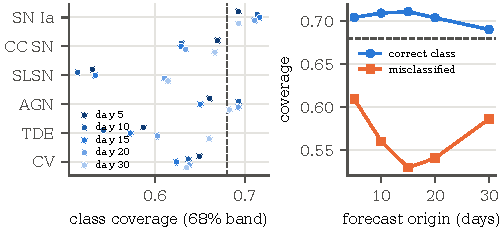
\includegraphics[width=\columnwidth]{figures/observation.pdf}
\caption{FLARE's 68\% bands on ZTF-BTS. Left: per-class coverage at each forecast origin. Right: coverage of correctly and incorrectly classified objects. Dashed: nominal.}
\label{fig:observation}
\end{figure}
